\documentclass[a4paper,12pt]{article}

%%% Работа с русским языком
\usepackage{cmap}					% поиск в PDF
\usepackage{mathtext} 				% русские буквы в формулах
\usepackage[T2A]{fontenc}			% кодировка
\usepackage[utf8]{inputenc}			% кодировка исходного текста
\usepackage[english,russian]{babel}	% локализация и переносы
\usepackage{xcolor}
\usepackage{hyperref}
 % Цвета для гиперссылок
\definecolor{linkcolor}{HTML}{799B03} % цвет ссылок
\definecolor{urlcolor}{HTML}{799B03} % цвет гиперссылок

\hypersetup{pdfstartview=FitH,  linkcolor=linkcolor,urlcolor=urlcolor, colorlinks=true}

%%% Дополнительная работа с математикой
\usepackage{amsfonts,amssymb,amsthm,mathtools} % AMS
\usepackage{amsmath}
\usepackage{icomma} % "Умная" запятая: $0,2$ --- число, $0, 2$ --- перечисление

%% Номера формул
%\mathtoolsset{showonlyrefs=true} % Показывать номера только у тех формул, на которые есть \eqref{} в тексте.

%% Шрифты
\usepackage{euscript}	 % Шрифт Евклид
\usepackage{mathrsfs} % Красивый матшрифт

%% Свои команды
\DeclareMathOperator{\sgn}{\mathop{sgn}}

%% Перенос знаков в формулах (по Львовскому)
\newcommand*{\hm}[1]{#1\nobreak\discretionary{}
{\hbox{$\mathsurround=0pt #1$}}{}}
% графика
\usepackage{graphicx}
\graphicspath{{pictures/}}
\DeclareGraphicsExtensions{.pdf,.png,.jpg}
\author{Бурмашев Григорий, БПМИ-208}
\title{Матан, дз -- 4}
\date{\today}
\begin{document}
\maketitle
\clearpage
\section*{Номер 1}
Вычислить:
\[
\lim_{p \rightarrow 0+ } \int\limits_{0}^{+\infty} \frac{xe^{-px}}{(x^2 + 1)^2} dx
\]
Проверяем условия для теоремы с сема:
\begin{center}
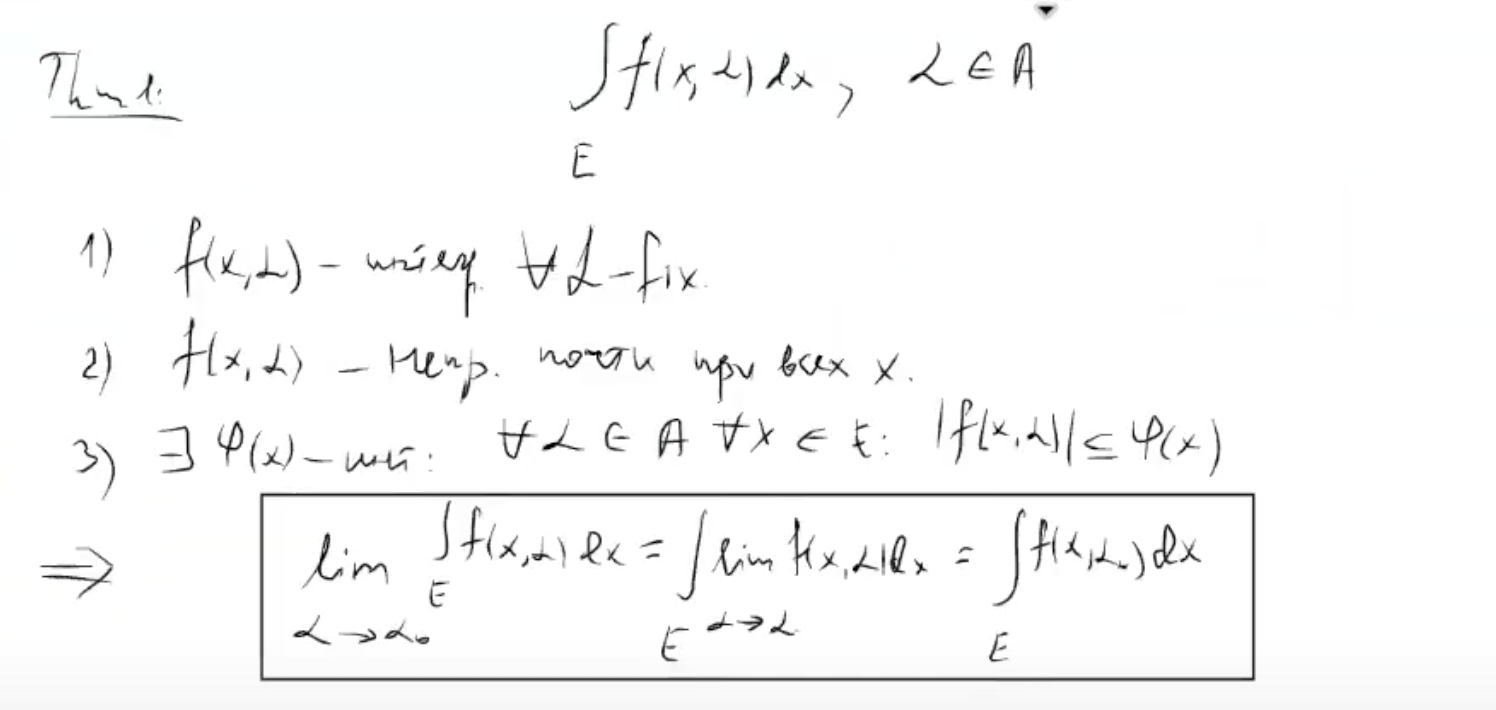
\includegraphics[scale=0.5]{5.png}
\end{center}
 Подинтегральная функция непрерывна для любого $x$. В знаменателе нет проблем, так как там везде квадраты. Из непрерывности получаем интегрируемость. Осталось подобрать мажорантную функцию для 3 пункта. Заметим, что у нас $p \rightarrow 0+$, а также $x \geq 0$, значит при таком $p$ \; $e^{-px}  \leq 1$, пробуем:
\[
\left|
\frac{xe^{-px}}{(x^2 + 1)^2}
\right|
\leq 
\frac{x \cdot 1}{(x^2 + 1)^2}
\]
Ну а эта функция тем более интегрируема. Все 3 условия выполняются, значит можем пользоваться теоремой:
\[
\lim_{p \rightarrow 0+ } \int\limits_{0}^{+\infty} \frac{xe^{-px}}{(x^2 + 1)^2} dx = 
 \int\limits_{0}^{+\infty}  \lim_{p \rightarrow 0+ } \frac{xe^{-px}}{(x^2 + 1)^2} dx = 
 \int\limits_{0}^{+\infty}  \frac{x}{(x^2 + 1)^2} dx = 
\]
\[
=
-\left(\frac{1}{2(x^2 + 1)}\right) \Bigg|_0^{+\infty} = 0 - \left(- \frac{1}{2}\right) = \frac{1}{2}
\]
\begin{center}
\textbf{Ответ: } 
\[
\frac{1}{2}
\]
\end{center}
\clearpage
\section*{Номер 2}
Найти область определения функции, заданной интегралом, и исследовать эту функцию на непрерывность:
\[
\int\limits_0^{\infty} \frac{\cos px}{\sqrt{1 + x^3}} dx
\]
Номер аналогичен 6 с семинара. Проверяем условия для теоремы с сема:
\begin{center}
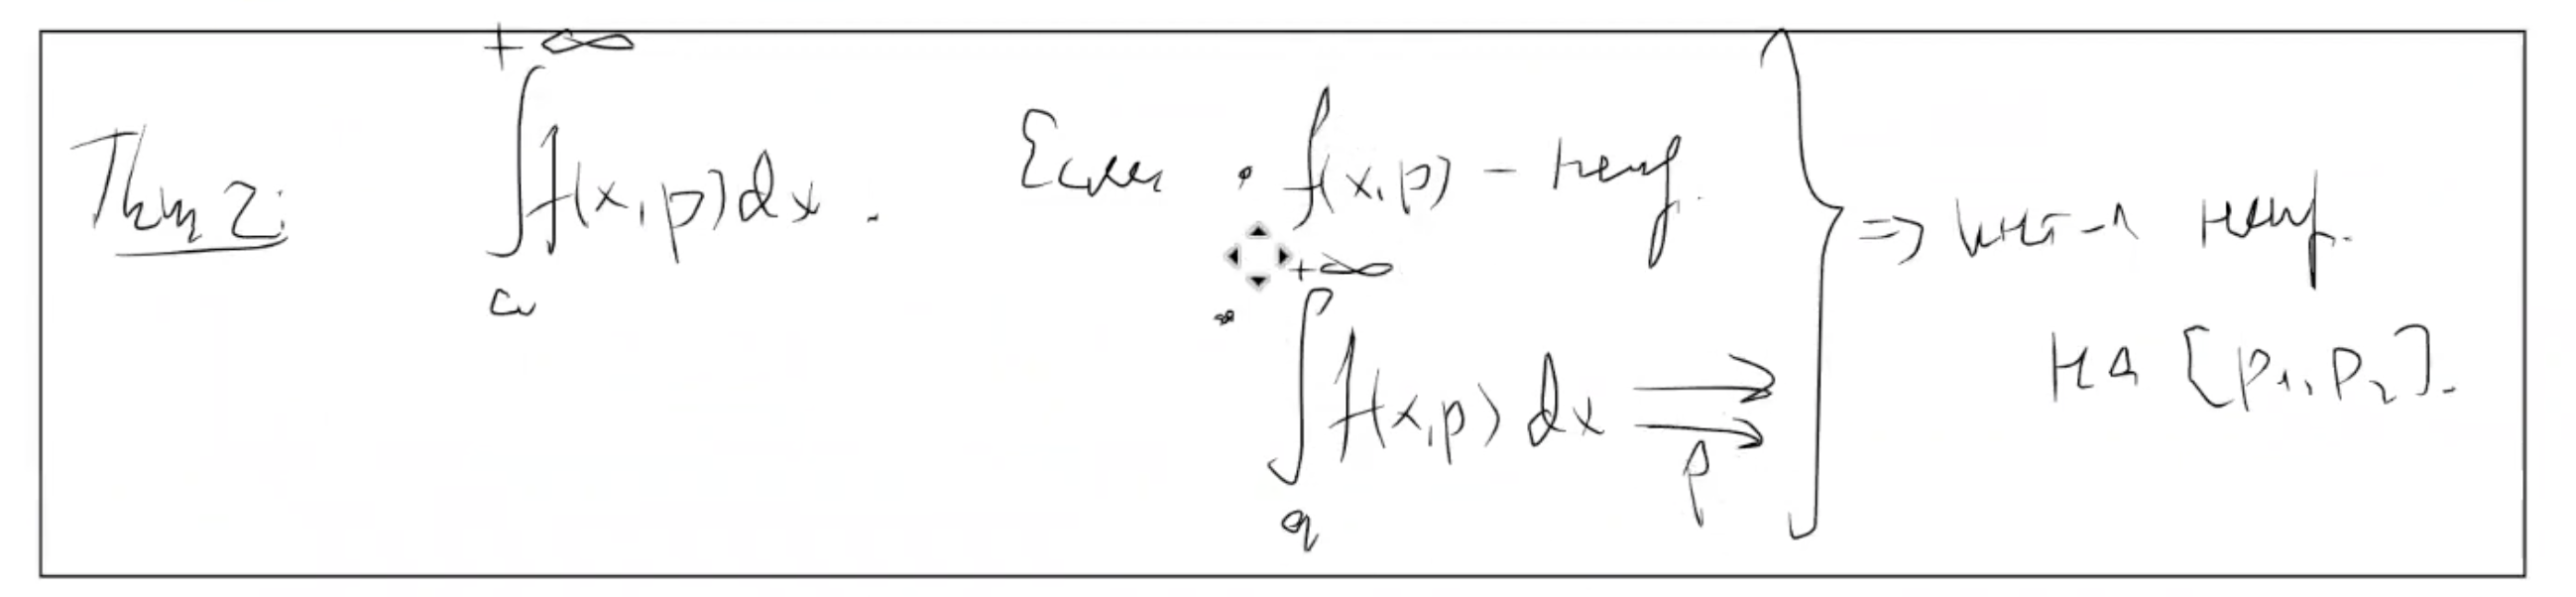
\includegraphics[scale=0.3]{6.png}
\end{center}
Разберемся для начала с областью определения. Попробуем по признаку Дирихле доказать, что интеграл сходится. Для начала разберемся с косинусом. Заметим, что при любых пределах интегрирования мы можем сказать:
\[
\left|
\int \cos  ( pt )dt 
\right|
\leq \frac{2}{p} 
- \text{ ограниченно}
\]
Но здесь возникает проблемный случай $p = 0$, так что рассмотрим его отдельно позже, пока что скажем, что $p \neq 0 $. Теперь посмотрим на вторую функцию $\frac{1}{\sqrt{1 + x^3}}$:
\[
\frac{1}{\sqrt{1 + x^3}} \rightarrow 0 \text{ монотонно }
\]
Из этих двух пунктов по обычному признаку Дирихле получаем, что наш интеграл сходится. Нужно вспомнить про $p = 0$, при нем:
\[
\int\limits_0^{\infty} \frac{1}{\sqrt{1 + x^3}} dx
\]
Этот интеграл сходится, а значит мы получаем область определения $\mathbb{R}$, т.е:
\[
p \in \mathbb{R}
\]
Теперь надо проверить непрерывность, проверяем:
\[
fix \;  \forall p \neq 0 \; : \; \exists \;  p_0 > 0 : \;  p \in [p_0, +\infty)
\]
Если $p$ отрицательное, то будет:
\[
fix \;  \forall p \neq 0 \; : \; \exists \;  p_0 > 0 : \;  p \in [-\infty, -p_0)
\]
Но поскольку все симметрично, будем рассматривать случай для положительных, проверяем:
\[
\left|
\int \cos  ( pt )dt 
\right|
\leq \frac{2}{p} 
\leq \frac{2}{p_0}
\text{ равномерно ограниченно}
\]
В знаменателе вообще нет параметра, поэтому там всё просто, он равномерно и монотонно стремится к нулю:
\[
\frac{1}{\sqrt{1 + x^3}} \rightrightarrows 0 \text{ монотонно }
\]
Теперь снова проверяем случай $p = 0$, при нем:
\[
\int\limits_0^{\infty} \frac{1}{\sqrt{1 + x^3}} dx  \text{ непрерывно }
\]
По признаку Дирихле для интегралов с параметром получаем равномерную сходимость на промежутке $[p_0, +\infty)$, следовательно функция непрерывна в любой фиксированной точке $p$, значит есть непрерывность везде, а значит есть непрерывность на $\mathbb{R}$
\begin{center}
\textbf{Ответ:} область определения $p \in \mathbb{R}$, там непрерывность есть
\end{center}
\clearpage
\section*{Номер 3}
Найти область определения функции, заданной интегралом, и исследовать эту функцию на непрерывность:
\[
\int\limits_0^1 \frac{\sin x}{x^p} dx
\]
Номер аналогичен 3 с семинара. Имеем проблемную точку $x = 0$, в остальном всё хорошо. Посмотрим, что происходит в окрестности нуля. Там $\sin x \sim x$, а значит: 
\[
\int\limits_0^{\varepsilon}   \frac{\sin x}{x^p} dx \sim
\int\limits_0^{\varepsilon}   \frac{x}{x^p} dx  = 
\int\limits_0^{\varepsilon}   \frac{1}{x^{p - 1}} dx
\]
Ну а мы знаем, что такой интеграл сходится при $p - 1 < 1$, т.е $p < 2$. Получили область определения. Теперь будем проверять непрерывность при таких $p$. Проверяем аналогично предыдущему номеру:
\[
\forall \; fix \; p < 2 \; : \; \exists \; p_0 : \; p < p_0 < 2\; : \text{ область } (0, 1) \times (-\infty, p_0)
\]
На этой области докажем равномерную сходимость:
\[
\int\limits_0^1 \frac{\sin x}{x^p} dx 
< 
\int\limits_0^1 \frac{\sin x}{x^{p_0}} dx 
\]
Ну а этот интеграл сходится, т.к $p_0 < 2$. А значит исходный интеграл сходится равномерно по признаку Вейерштрасса на области $p \in (-\infty, p_0)$. Значит непрерывна в выбранной фиксированной точке $p < 2$, а следовательно непрерывно $\forall p < 2$.
\begin{center}
\textbf{Ответ: } область определения $p < 2$, там непрерывность есть
\end{center}
\clearpage
\section*{Номер 4}
Вычислить интегралы
\subsection*{a)}
\[
\int\limits_0^{+\infty} \frac{\sin x^3}{x} dx
\]
Нужно свести к интегралу Дирихле, поэтому введем замену:
\[
\int\limits_0^{+\infty} \frac{\sin x^3}{x} dx
=
\begin{bmatrix}
t = x^3 \\ 
x = \sqrt[3]{t} \\
dt = 3x^2 dx \\
dx = \frac{dt}{3x^2}
\end{bmatrix} =
\int\limits_0^{+\infty} \frac{\sin t}{\sqrt[3]{t}} \frac{dt}{3\sqrt[3]{t^2}} =
\int\limits_0^{+\infty} \frac{1}{3} \cdot \frac{\sin t}{\sqrt[3]{t^3}} dt =
\]
\[
=
\frac{1}{3}\int\limits_0^{+\infty}  \frac{\sin t}{t} dt 
=
\frac{1}{3} \cdot \frac{\pi}{2} = \frac{\pi}{6}
\]
\begin{center}
\textbf{Ответ: } 
\[
\frac{\pi}{6}
\]
\end{center}
\subsection*{b)}
\[
\int\limits_0^{+\infty} \frac{\cos^2 x}{9 + x^2} dx
\]
Похоже на интеграл Лапласа, только вместо $1$ имеем $9$, это, в свою очередь, похоже на 9 номер с семинара.
\[
\int\limits_0^{+\infty} \frac{\cos^2 x}{9 + x^2} dx
=
\frac{1}{9} 
\int\limits_0^{+\infty} \frac{\cos^2 x}{1 + \left(\frac{x}{3}\right)^2} dx
\]
Понизим степень у косинуса, чтобы избавиться от квадрата:
\[
=
\frac{1}{9} 
\int\limits_0^{+\infty} \frac{\frac{1 + \cos 2x}{2}}{1 + \left(\frac{x}{3}\right)^2} dx
=
\frac{1}{18} 
\int\limits_0^{+\infty} \frac{1 + \cos 2x}{1 + \left(\frac{x}{3}\right)^2} dx
=
\]
\[
=
\frac{1}{18} 
\left( 
\int\limits_0^{+\infty} \frac{1}{1 + \left(\frac{x}{3}\right)^2} dx
+
\int\limits_0^{+\infty} \frac{\cos 2x}{1 + \left(\frac{x}{3}\right)^2} dx
\right)
\]
Разберемся по отдельности, левый интеграл очевный:
\[
\int\limits_0^{+\infty} \frac{1}{1 + \left(\frac{x}{3}\right)^2} dx 
=
3
\int\limits_0^{+\infty} \frac{1}{1 + t^2} dt
=
3\arctg \left(t\right) \Bigg|_0^{+\infty}  = 3\frac{\pi}{2} - 0 = \frac{3\pi}{2} 
\]
Правый интеграл есть интеграл из 9 номера из семинара, на всякий случай прикладываю:
\begin{center}
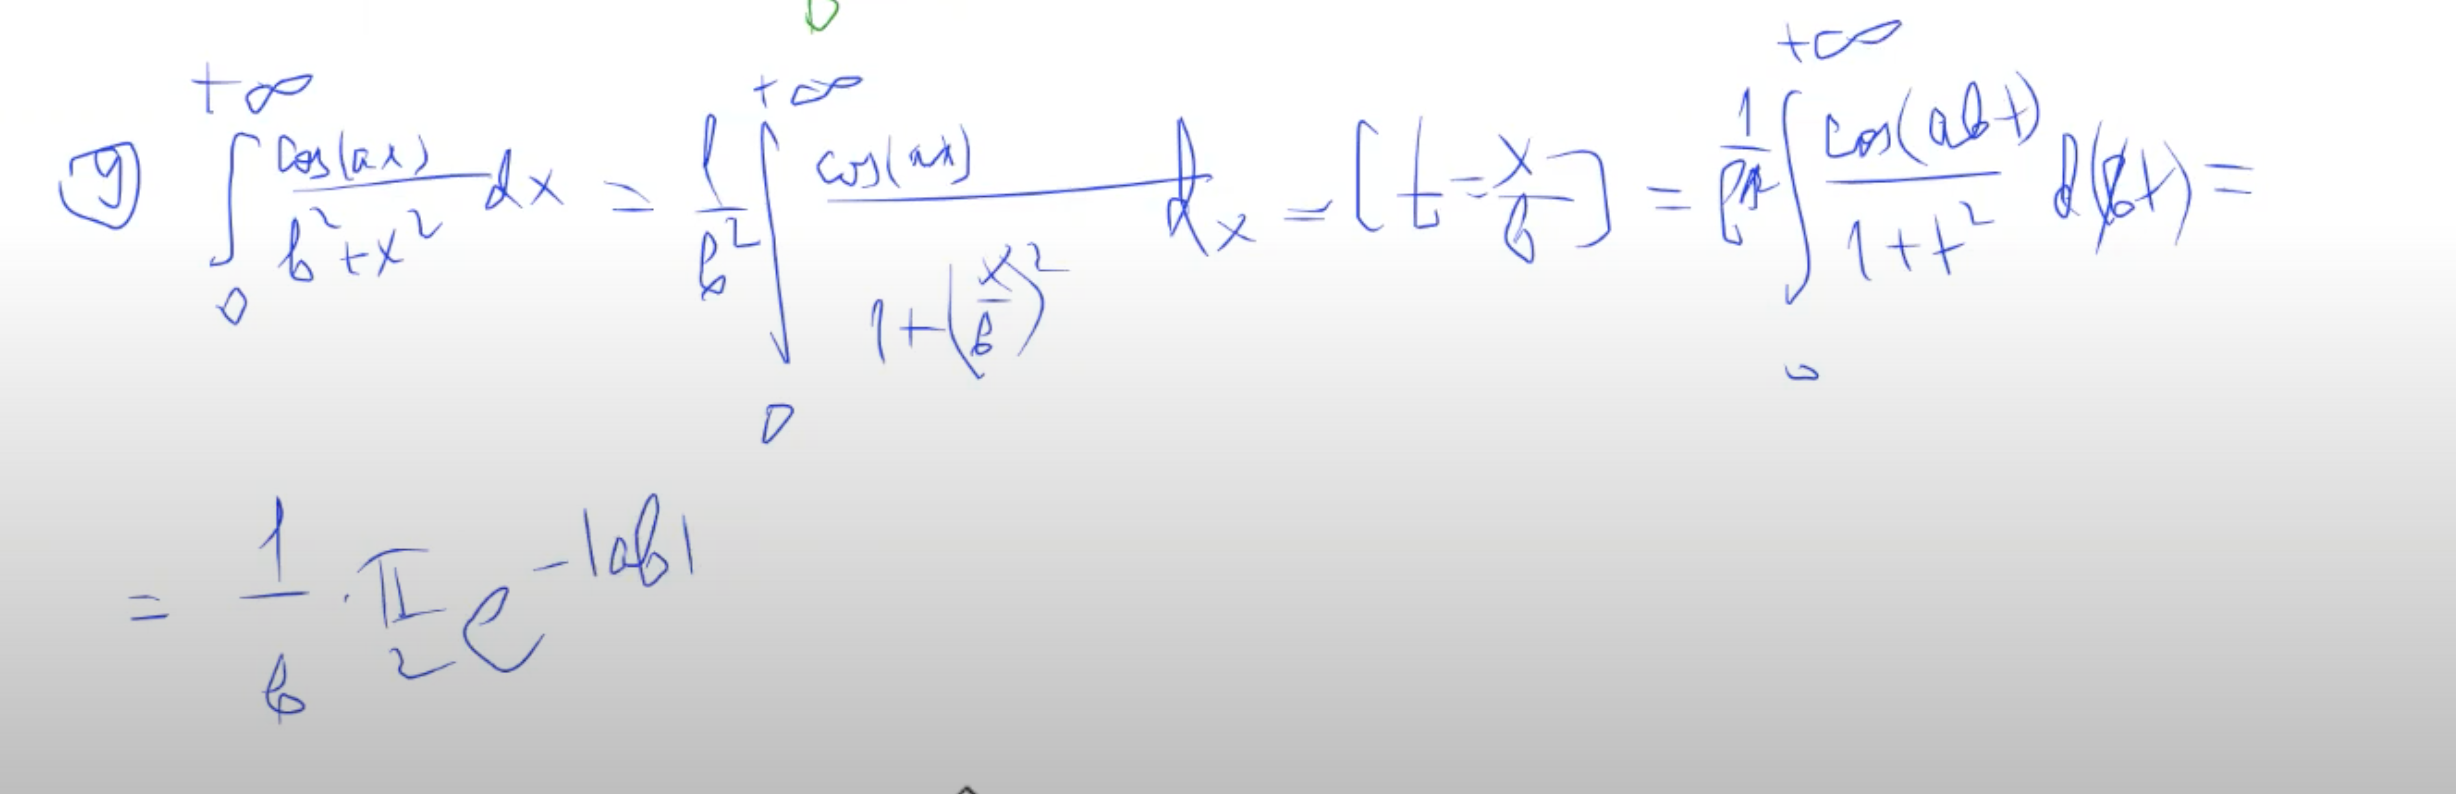
\includegraphics[scale=0.3]{7.png}
\end{center}
Так что получаем:
\[
\int\limits_0^{+\infty} \frac{\cos 2x}{1 + \left(\frac{x}{9}\right)^2} dx = 
\int\limits_0^{+\infty} \frac{9\cos 2x}{9 + x^2} dx = 9 \cdot \int\limits_0^{+\infty} \frac{\cos 2x}{9 + x^2} dx  =
9 \cdot \left(
\frac{1}{3} \cdot \frac{\pi}{2} \cdot e^{-|2 \cdot 3|}
=
\frac{3\pi}{2} \cdot e^{-6}
\right)
\]
Возвращаемся к исходному интегралу и подставляем:
\[
\frac{1}{18} \left(
\frac{3\pi}{2} + \frac{3\pi}{2} \cdot e^{-6}
\right)
=
\frac{\pi}{12} + \frac{\pi}{12} \cdot e^{-6} = \frac{\pi}{12} \cdot (1 + e^{-6})
\]
\begin{center}
\textbf{Ответ: } 
\[
\frac{\pi}{12} \cdot (1 + e^{-6})
\]                               
\end{center}
\end{document}
